\begin{frame}[fragile]{Tutorial: n-site states with MPS}

\begin{columns}

\begin{column}{6cm}

\begin{onlyenv}<1->
\begin{lstlisting}[language=JuliaLocal, style=julia, mathescape, basicstyle=\small]
  j = n ÷ 2
  X$_j$ = op("X", i[j])

  X$_j$Zp = apply(X$_j$, Zp)


  state = [k == j ? "Z-" : "Z+"
                           for k in 1:n]
  X$_j$Zp = MPS(i, state)
\end{lstlisting}
\end{onlyenv}

\begin{onlyenv}<3->
\begin{lstlisting}[language=JuliaLocal, style=julia, mathescape, basicstyle=\small]
  maxlinkdim(X$_j$Zp) == 1
  inner(Zp, X$_j$Zp) == 0
\end{lstlisting}
\end{onlyenv}

\end{column}

\begin{column}{4.5cm}

\begin{onlyenv}<1-1>
~\\
~\\
~\\
$X_j|Z+Z+\dots Z+\rangle =$ \\
$|Z+Z+\dots Z-\dots Z+\rangle$ \\
~\\
~\\
$|Z+Z+\dots Z-\dots Z+\rangle$ \\
~\\
\end{onlyenv}

\begin{onlyenv}<2->
\vspace*{0.0cm}
\begin{center}
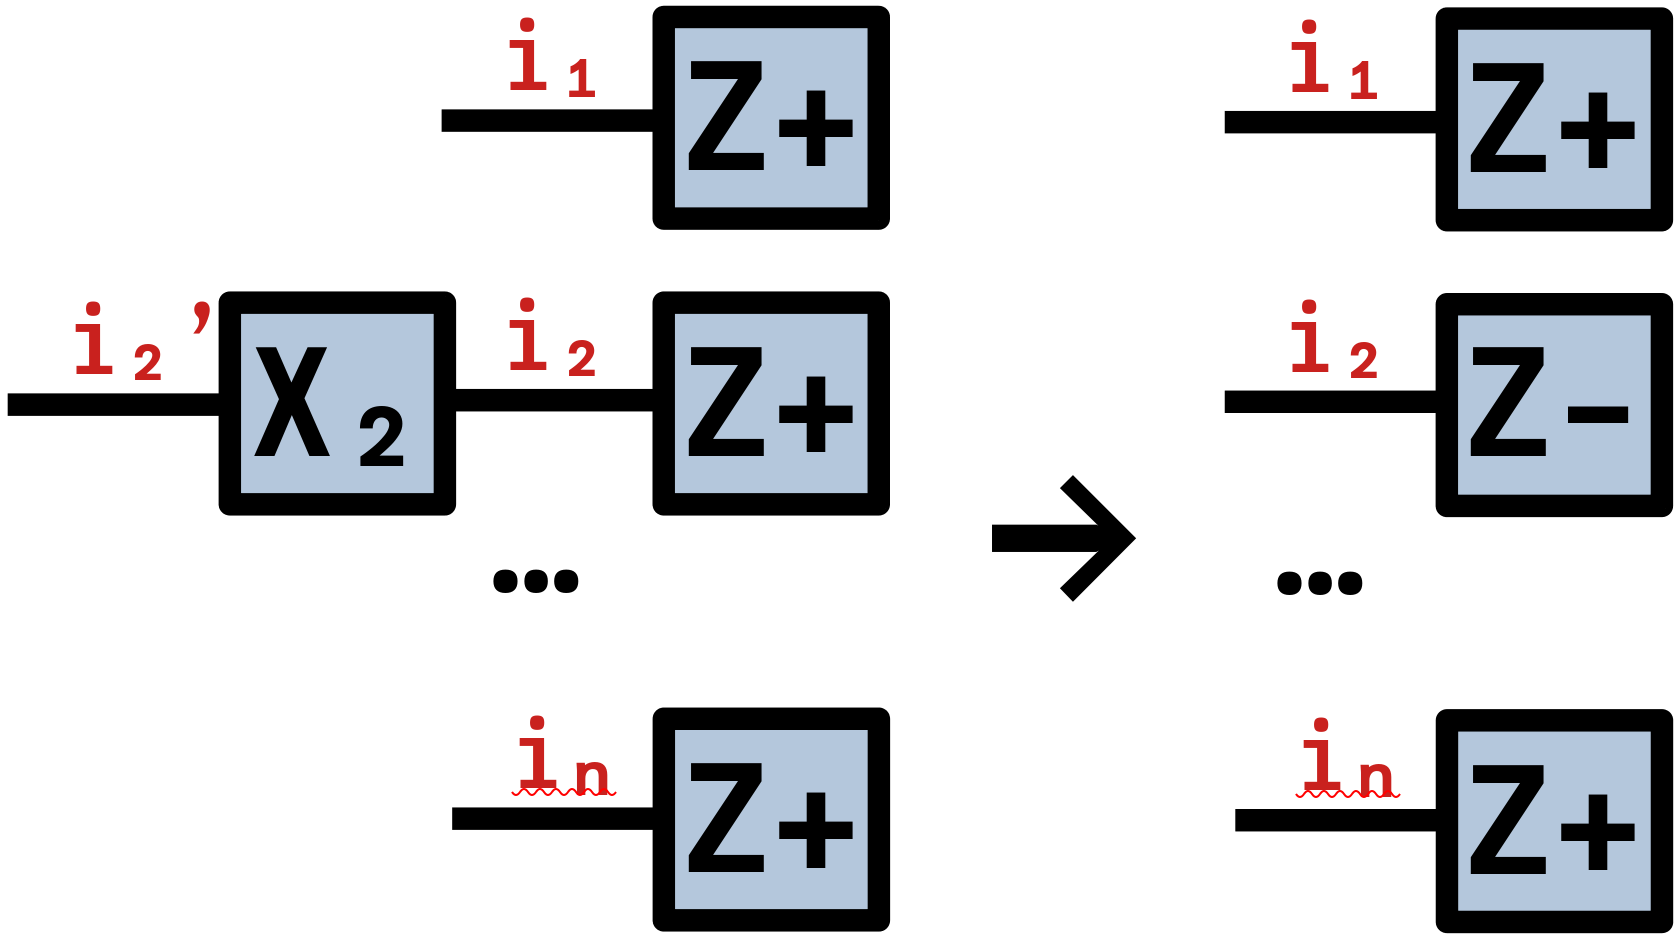
\includegraphics[width=1.0\textwidth]{
  slides/assets/XjZpn.png
}
\end{center}
\vspace*{0.0cm}
\end{onlyenv}

\begin{onlyenv}<3->
~\\
~\\
~\\
~\\
~\\
\end{onlyenv}

\end{column}

\end{columns}

\end{frame}
